\documentclass[letterpaper, 11pt]{article}
%\usepackage[hmargin = 1in, vmargin = 1in]{geometry}
\usepackage{amsmath}
\usepackage{amssymb}
\usepackage{enumitem}
\usepackage{mathrsfs}
\usepackage{tikz}
\usepackage{graphicx}
\usepackage{algorithmicx}
\usepackage{algpseudocode}
% \doublespacing
\setlength{\headheight}{14pt}
\usepackage{fancyhdr}
\pagestyle{fancy}
\rhead{Gabriel Wallace}
\lhead{Comp Sci 3130}

\newcommand{\card}{\text{Card}}
\newcommand{\N}{\mathbb{N}}
\newcommand{\R}{\mathbb{R}}
\newcommand{\Z}{\mathbb{Z}}
\newcommand{\Q}{\mathbb{Q}}

\newcommand{\inv}{^{-1}}
\newcommand{\abs}[1]{\lvert #1 \rvert}
\newcommand{\hwnumber}[3]{\medskip \noindent\textbf{#1.} Section #2 \##3 \smallskip}
\newcommand{\Mod}[1]{\ \mathrm{mod}\ #1}

\begin{document}
\begin{center}
	{\LARGE Homework 1}\\
\end{center}

\hwnumber{1}{1.1}{6}

\begin{enumerate}[label = (\alph*)]
  \item We find $\gcd(31415, 14142)$ by Euclid's Algorithm.
    \begin{align*}
      \gcd(31415, 14142) &= \gcd(14142, 3131)\\
                         &= \gcd(3131, 1618)\\
                         &= \gcd(1618, 1513)\\
                         &= \gcd(1513, 105)\\
                         &= \gcd(105, 43)\\
                         &= \gcd(43, 19)\\
                         &= \gcd(19, 5)\\
                         &= \gcd(5, 4)\\
                         &= \gcd(4, 1)\\
                         &= \gcd(1, 0)\\
                         &= 1
    \end{align*}

  \item We see that the number of iterations for Euclid's algorithm is 11. The
    number of iterations for the method of consecutive integers is 14142, or
    approximately 1286 times faster. 

    Writing a quick Python program to run one million simulations reveals that,
    on average, Euclid's algorithm takes about 11 iterations and the consecutive
    integers method takes about 39960 iterations, or about 3633 times faster.
\end{enumerate}

\hwnumber{2}{1.1}{8}

Let $m, n \in \Z$ with $m < n$. Applying Euclid's algorithm, we have $\gcd(m, n)
= \gcd(n, m \Mod{n})$. But since $m < n$, then $m \Mod{n} = m$, so $\gcd(n, m
\Mod{n}) = \gcd(n, m)$. In other words, the two inputs are swapped. 

The inputs swapping can only happen on the first iteration and if $m < n$. For
any integers $a$ and $b$, $a > b \Mod{a}$, since $b \Mod{a}$ is the
remainder of $b$ when divided by $a$ and the remainder is smaller than the
quotient, by the Division Algorithm. 

\newpage

\hwnumber{3}{1.2}{3}

Only (a) is an algorithm (provided we know how to compute a square root). The
problems with (b) and (c) is that they are ambiguous, i.e we are not given how
to compute $A$ or $h_a$ respectively. 

\hwnumber{4}{1.2}{5}

\begin{enumerate}[label = (\alph*)]
  \item Let $n$ be a positive integer and let $r = n - 2a$, where $a$ is 
    a positive integer. Then prepend $r$ to the binary representation of 
    $n$. Then assign $n$ to $a$ and repeat this process until $n = 0$. 

  \item 
    \begin{algorithmic}
      \State //Input: an integer of size $n$
      \State //Output: the binary representation of $n$ represented by the list 
      $d_k, d_{k-1}, \dots, d_1, d_0$
      \State
      \State $k\gets 0$
      \While {$n \not= 0$}
        \State $b_k \gets n \Mod 2$
        \State $n \gets \lfloor \frac{n}{2} \rfloor$
        \State $k \gets k + 1$
      \EndWhile
    \end{algorithmic}


\end{enumerate}


\hwnumber{5}{1.3}{4}

\begin{enumerate}[label = (\alph*)]
  \item Let the two islands and the two banks of the river be the vertices and the
    bridges be the edges of a graph. Now we reformulate the question in graph
    theoretic terms: does this graph have an Euler cycle?

   \item The graph is below:

     \begin{center}
     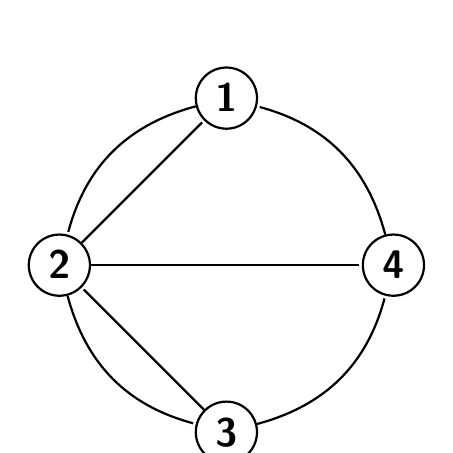
\begin{tikzpicture}[shorten >=1pt,auto,node distance=3cm,
                    thick,main node/.style={circle,draw,font=\sffamily\Large\bfseries}]

       \node[main node] (1) {1};
       \node[main node] (2) [below left of=1] {2};
       \node[main node] (3) [below right of=2] {3};
       \node[main node] (4) [below right of=1] {4};

       \path[every node/.style={font=\sffamily\small}]
         (1) edge [bend right] node[left] { } (2)
         (2) edge node [right] {} (1)
             edge node {} (4)
             edge [bend right] node[left] {} (3)
         (3) edge node [right] {} (2)
             edge [bend right] node[right] {} (4)
         (4) edge [bend right] node[right] {} (1);
     \end{tikzpicture}
   \end{center}

    From graph theory we have a theorem:
    A (connected) graph has an Euler cycle if and only if every vertex has even
    degree. In this graph, every vertex has an odd degree. So, we need to build
    two more edges: one connecting (1) and (3) and the other connecting (2)
    and (4). If all we care about is an Eulerian path (that is we only care
    about traversing every edge and our starting and stopping point does not
    matter), then just one extra edge would suffice. 
\end{enumerate}

\hwnumber{6}{1.3}{8}

\begin{enumerate}[label = (\alph*)]
  \item We first translate this map into a graph with each region being a vertex
    and two vertices are connected if they share an edge on the map. Doing so,
    we have the following graph:

    \begin{center}
    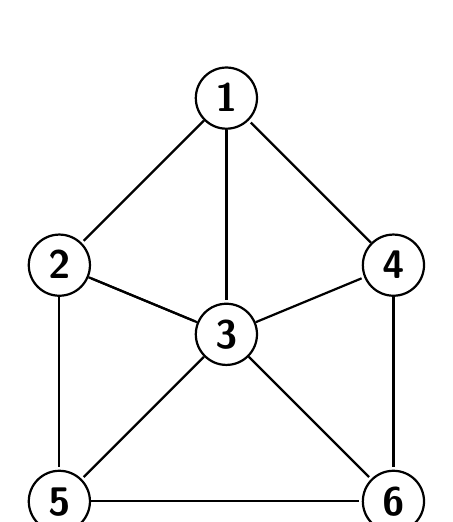
\begin{tikzpicture}[shorten >=1pt,auto,node distance=3cm,
                    thick,main node/.style={circle,draw,font=\sffamily\Large\bfseries}]

       \node[main node] (1) {1};
       \node[main node] (2) [below left of=1] {2};
       \node[main node] (3) [below of=1] {3};
       \node[main node] (4) [below right of=1] {4};
       \node[main node] (5) [below left of=3] {5};
       \node[main node] (6) [below right of=3] {6};


       \path[every node/.style={font=\sffamily\small}]
         (1) edge [right] node[left] {} (2)
             edge node {} (3)
         (2) edge node {} (3)
             edge node {} (5)
         (3) edge node [right] {} (2)
             edge [right] node[right] {} (4)
             edge node {} (5)
             edge node {} (6)
         (4) edge [right] node[right] {} (1)
             edge node {} (6)
         (5) edge node {} (6);
      
    \end{tikzpicture}
  \end{center}


  \item We can color the graph with four colors like so:
    \begin{figure}[h!]
      \centering
      \includegraphics[width=0.3\linewidth]{4_colors.png}
    \end{figure}

\end{enumerate}


\hwnumber{7}{2.1}{1}

\begin{enumerate}[label = (\alph*)]
  \item Computing the sum of $n$ numbers
    \begin{enumerate}[label=(\roman*)]
      \item $n$
      \item Addition of two numbers
      \item No
    \end{enumerate}
  \item Computing $n!$
    \begin{enumerate}[label=(\roman*)]
      \item $n$
      \item Multiplication of two integers
      \item No
    \end{enumerate}
  \item Finding the largest element in a list of $n$ numbers
    \begin{enumerate}[label=(\roman*)]
      \item $n$
      \item Comparison of two objects
      \item No
    \end{enumerate}
\end{enumerate}

\hwnumber{8}{2.1}{2(a)}

The basic operation is addition of two numbers. Let $T$ be the total number of
operations and let $N$ be the total number of elements in the two matrices.
Since the number of elements of an $n \times n$ matrix is $n^2$, then $N =
2n^2$. And since we add two matrices straight across, $T = n^2$. Therefore, $T =
N / 2$. 

\hwnumber{9}{2.1}{4(a)}

In the best case, we would get lucky and select a matching pair in the first two
selections. So the smallest number of gloves selected is 2. 

In the worst case, we would select every glove of a particular handedness, so we
would have 11 gloves. In the next selection, we would be guaranteed a match. So
the largest number of gloves selected is 12. 


\hwnumber{Bonus}{1.2}{2}

The order of traversals that will take 17 minutes is as follows:

\begin{center}
  \begin{tabular}{c | c | c}
    People sent & Time taken & Total time \\
    \hline
    1, 2 & 2 min & 2 min \\ 
    2 & 2 min & 4 min \\
    3, 4 & 10 min & 14 min \\
    1 & 1 min & 15 min \\
    1, 2 & 2 min & 17 min \\
  \end{tabular}
\end{center}

\end{document}
